\documentclass[12pt,letterpaper]{article}

% Paquetes base
\usepackage[spanish]{babel}
\usepackage[utf8]{inputenc}
\usepackage[T1]{fontenc}
\usepackage{mathpazo}
\usepackage[margin=2.5cm]{geometry}
\usepackage{setspace}
\onehalfspacing
\usepackage{parskip}
\usepackage{microtype}
\usepackage{graphicx}
\usepackage{hyperref}

\hypersetup{colorlinks=false, linkcolor=black, urlcolor=blue, citecolor=black}
\usepackage{array}    
\usepackage{booktabs} 
\usepackage{caption}  
\usepackage{xcolor}
\usepackage{enumitem}
\usepackage{ragged2e}
\usepackage{float}
\usepackage{csquotes}
\usepackage{tabularx}
\usepackage{booktabs}
\usepackage{multirow}
\usepackage{amsmath}
\usepackage{amssymb}
\newcommand{\tvhead}[1]{\textbf{#1}}
\newcommand{\boolnot}[1]{\ensuremath{\overline{#1}}}
\usepackage{tikz}

\addto\captionsspanish{\renewcommand{\refname}{Bibliografía}}

% Encabezado/pie
\usepackage{fancyhdr}
\pagestyle{fancy}
\fancyhf{}

% Altura del encabezado para que quepa el logo (1.8 cm ~ 51pt)
\setlength{\headheight}{52pt}
% (Opcional) si ves el contenido muy abajo, puedes recuperar un poco de margen:
% \addtolength{\topmargin}{-8pt}

% Encabezado
\lhead{
\includegraphics[height=1.8cm]{Img/escudo.png}}
\chead{Universidad del Bío-Bío}
%\rhead{\nouppercase{\leftmark}}

% Pie de página
\lfoot{Sistemas Digitales}
\cfoot{\thepage}
\rfoot{Grupo 8}

% Líneas superior e inferior
\renewcommand{\headrulewidth}{0.4pt}
\renewcommand{\footrulewidth}{0.4pt}

% Espaciado de títulos (aleja los títulos del encabezado)
\usepackage{titlesec}
\titleformat{\section}{\normalfont\Large\bfseries\filcenter}{\thesection}{1em}{}
\titlespacing*{\section}{0pt}{1cm}{-0.1cm}
\titlespacing*{\subsection}{0pt}{1cm}{-0.1cm}

% (Opcional) Sin numeración en títulos (y siguen en el índice)
%\setcounter{secnumdepth}{0}

% (Opcional) Cambiar el nombre del índice a "Índice"
\addto\captionsspanish{\renewcommand{\contentsname}{Índice}}
\renewcommand{\thetable}{\arabic{table}}
\renewcommand{\thefigure}{\arabic{figure}}
\setlength{\footskip}{0.9cm}  % valor más chico → sube el pie

\begin{document}
	
	\begin{titlepage}
		\thispagestyle{empty}
		
		% ===== Bloque superior: escudo + institución =====
		\begin{center}
			\vspace*{-2cm} % margen superior discreto
			
\includegraphics[height=3.5cm]{Img/escudo.png}\\[-0.2cm]
			
			{\large Universidad del Bío-Bío}\\[-2pt]
			{\large Facultad de Ciencias Empresariales}\\[-2pt]
			{\large Ingeniería Civil en Informática}
		\end{center}
		
		\vspace{1cm}
		\vfill
		
		% ===== Bloque central: TÍTULO =====
		\begin{center}
			\rule{\textwidth}{0.5pt}\\[0.5cm]
			{\Huge \textbf{Informe de laboratorio N\textsuperscript{o}4}}\\[0.25cm]
			{\Large Operaciones Lógicas}\\[0.1cm]
			\rule{0.65\textwidth}{0.5pt}
		\end{center}
		
		\vspace{2cm}
		
    \begin{flushleft}
    \normalsize
    \begin{tabular}{@{}ll@{}}
                           & \\
    \textbf{Integrantes}   & : Oscar Illanes Garrido \\
                           & \hspace{0.12 cm} Gabriela Maureira Ocaña \\
                           & \hspace{0.12 cm}  Bastian Palma Navarrete \\
                           & \\
    \textbf{Docente}       & : Julio C. Alarcón Monteros \\
                           & \\
    \textbf{Asignatura}    & : Sistemas Digitales \\
                           & \\
    \textbf{Carrera}    & : Ingeniería Civil en Informática \\
    \end{tabular}
    \end{flushleft}
		
		\vfill
		\begin{center}
			\normalsize\textbf{Chillán, 5 de junio de 2026.}
		\end{center}
	\end{titlepage}
	
	\tableofcontents 

	\newpage
	\section{Introducción}

    En los sistemas digitales, la información se representa mediante niveles lógicos binarios, permitiendo procesar datos a través de circuitos electrónicos formados por compuertas lógicas. Estas compuertas constituyen la base del funcionamiento de computadores, sistemas de control, dispositivos de comunicación y una gran variedad de aplicaciones tecnológicas actuales. A partir de combinaciones de señales de entrada es posible obtener respuestas específicas mediante operaciones lógicas definidas.

    Dentro de este contexto, las compuertas AND, OR, NAND y NOT permiten implementar circuitos combinacionales capaces de generar distintas salidas según las condiciones presentes en sus entradas. El análisis de estos circuitos puede realizarse mediante expresiones booleanas y tablas de verdad, herramientas que permiten representar y comprender su funcionamiento. Además, mediante la aplicación de las propiedades y teoremas del álgebra de Boole, es posible simplificar las expresiones obtenidas, reduciendo la cantidad de compuertas necesarias sin modificar el comportamiento del circuito.

    El estudio de circuitos lógicos combinacionales considera la obtención de expresiones booleanas, la construcción de tablas de verdad y la verificación de su funcionamiento mediante simulación. Asimismo, la aplicación de técnicas de simplificación permite obtener circuitos equivalentes utilizando una menor cantidad de compuertas, manteniendo los mismos resultados para las distintas combinaciones de entrada.

    El presente informe se organiza comenzando con los objetivos planteados para la actividad. Posteriormente, se desarrolla el marco teórico relacionado con las compuertas lógicas, la lógica TTL y los métodos de simplificación. Luego se presenta el diseño del circuito, incluyendo el análisis del circuito original, la obtención de la tabla de verdad y el proceso de reducción de expresiones. Finalmente, se muestran los resultados obtenidos mediante simulación en el software NI Multisim y se comparan los resultados del circuito original y del circuito simplificado para comprobar su correcto funcionamiento.



    \section{Objetivo general:}
    
    \subsection{Objetivos específicos:}
    \begin{itemize}
        \item 
    \end{itemize}

    %========================================================================================
    \newpage
    \section{Desarrollo teórico}
    \subsection{Introducción a los sistemas digitales}
    Los sistemas digitales modernos operan fundamentalmente mediante el procesamiento de señales binarias donde la información se representa únicamente a través de dos estados lógicos: que podríamos definir como true(1) y false(0). Para manipular esta información se utilizan dispositivos llamados compuertas lógicas, las cuales implementan físicamente las  operaciones del álgebra de Boole y constituyen los bloques constructivos esenciales de cualquier circuito digital.
    
    \subsection{Compuertas lógicas}
    Las compuertas lógicas son dispositivos electrónicos que realizan operaciones booleanas sobre una o mas entradas digitales para producir una única salida digital. Según Floyd(2006), una compuerta lógica es un circuito electrónico que opera con señales binarias y cuyo comportamiento queda completamente descrito por su tabla de verdad.
    Cada compuerta implementa una función del álgebra de Boole, y puede describirse mediante tres elementos: su tabla de verdad, su expresión booleana y su símbolo lógico estándar.

    \subsubsection{Compuerta AND}
    La compuerta AND produce una salida de true (1) únicamente cuando todas sus entradas son true de forma simultánea. Para cualquier otra combinación, la salida es false (0). Su expresión booleana para dos entradas es:
    \begin{equation}
        S = A \cdot B
    \end{equation}
    En lógica TTL, la compuerta AND se implementa con transistores en configuración de colector común. La salida permanece en un nivel bajo mientras al menos una entrada esté en nivel bajo, actuando como un interruptor en serie.
    \newpage
    \vspace{0.3cm}
    \begin{center}
    \begin{tabular}{>{\centering\arraybackslash}p{1.5cm}
                    >{\centering\arraybackslash}p{1.5cm}
                    >{\centering\arraybackslash}p{2.5cm}}
    \toprule
    \tvhead{A} & \tvhead{B} & \tvhead{$S = A \cdot B$} \\
    \midrule
    0 & 0 & 0 \\
    0 & 1 & 0 \\
    1 & 0 & 0 \\
    1 & 1 & 1 \\
    \bottomrule
    \end{tabular}
    \captionof*{table}{Tabla de verdad – Compuerta AND}
    \end{center}
    \subsubsection{Compuerta OR}
    La compuerta OR produce una salida true (1) cuando al menos una de sus entradas es alta. Solo entrega salida false (0) cuando todas sus entradas son false. Su expresión booleana es:
    \begin{equation}
        S = A + B
    \end{equation}
    En lógica TTL, la compuerta OR se implementa con transistores en configuración paralelo, donde la presencia del nivel alto en cualquier transistor conduce la corriente y eleva la salida a nivel alto.
    \vspace{0.3cm}
    \begin{center}
        
    \begin{tabular}{>{\centering\arraybackslash}p{1.5cm}
                    >{\centering\arraybackslash}p{1.5cm}
                    >{\centering\arraybackslash}p{2.5cm}}
    \toprule
    \tvhead{A} & \tvhead{B} & \tvhead{$S = A + B$}\\
    \midrule
    0 & 0 & 0 \\
    0 & 1 & 1\\
    1 & 0 & 1\\
    1 & 1 & 1 \\
    \bottomrule
    \end{tabular}
    \captionof*{table}{Tabla de verdad – Compuerta OR}
    \end{center}
    \subsubsection{Compuerta NOT (Inversor)}
    La compuerta NOT o inversor tiene una única entrada y produce a la salida el complemento lógico de esta. Su expresión booleana es:
    \begin{equation}
    S = \boolnot{A}
    \end{equation} 
    En TTL, el inversor se implementa con un transistor en configuración emisor común.
    Cuando la entrada es true, el transistor cambia la salia a false; cuando la entrada es false, se cambia a true.
    \vspace{0.3cm}
    \begin{center}
        
    \begin{tabular}{>{\centering\arraybackslash}p{1.5cm}
                    >{\centering\arraybackslash}p{2.5cm}}
    \toprule
    \tvhead{A} & \tvhead{$S = \boolnot{A}$} \\
    \midrule
    0 & 1 \\
    1 & 0 \\
    \bottomrule
    \end{tabular}
    \captionof*{table}{Tabla de verdad – Compuerta NOT}
    \end{center}
    \subsubsection{Compuerta NAND}
    La compuerta NAND es la combinación de una AND seguida de un inversor. Entrega salida
    false (0) únicamente cuando todas sus entradas son true; en cualquier otro caso
    la salida es true (1). Su expresión booleana es:
    
    \begin{equation}
    S = \boolnot{A \cdot B}
    \end{equation}
    
    La NAND es considerada una compuerta universal, ya que cualquier función lógica
    puede implementarse utilizando únicamente compuertas NAND. En TTL es la compuerta más
    común porque su implementación con transistores BJT es directa y eficiente.
    
    \vspace{0.3cm}
    \begin{center}
    \begin{tabular}{>{\centering\arraybackslash}p{1.5cm}
                    >{\centering\arraybackslash}p{1.5cm}
                    >{\centering\arraybackslash}p{2.5cm}}
    \toprule
    \tvhead{A} & \tvhead{B} & \tvhead{$S = \boolnot{A \cdot B}$} \\
    \midrule
    0 & 0 & 1 \\
    0 & 1 & 1 \\
    1 & 0 & 1 \\
    1 & 1 & 0 \\
    \bottomrule
    \end{tabular}
    \captionof*{table}{Tabla de verdad – Compuerta NAND}
    \end{center}
    \newpage

    \subsection{Compuerta NOR}
    
    La compuerta NOR es la combinación de una OR seguida de un inversor. Entrega salida true
    (1) únicamente cuando todas sus entradas son false. Al igual que la NAND, la NOR
    también es una compuerta universal. Su expresión booleana es:
    
    \begin{equation}
    S = \boolnot{A + B}
    \end{equation}
    
    \vspace{0.3cm}
    \begin{center}
    \begin{tabular}{>{\centering\arraybackslash}p{1.5cm}
                    >{\centering\arraybackslash}p{1.5cm}
                    >{\centering\arraybackslash}p{2.5cm}}
    \toprule
    \tvhead{A} & \tvhead{B} & \tvhead{$S = \boolnot{A + B}$} \\
    \midrule
    0 & 0 & 1 \\
    0 & 1 & 0 \\
    1 & 0 & 0 \\
    1 & 1 & 0 \\
    \bottomrule
    \end{tabular}
    \captionof*{table}{Tabla de verdad – Compuerta NOR}
    \end{center}

    \subsection{Lógica TTL (Transistor-Transistor Logic)}
    
    La lógica TTL es una familia de circuitos integrados digitales basada en transistores
    bipolares de unión (BJT). Fue introducida en la década de 1960 y se convirtió en el
    estándar de facto de la electrónica digital durante décadas. Según Floyd~(2006), los
    circuitos TTL se caracterizan por operar con una tensión de alimentación de $+5\,\text{V}$
    y por definir los niveles lógicos de la siguiente manera:
    
    \begin{itemize}[leftmargin=1.5cm]
    \item Nivel lógico alto (1): Voltaje de salida típico entre 2{,}4~V y 5~V.
    \item Nivel lógico bajo (0): Voltaje de salida típico entre 0~V y 0{,}4~V.
    \item Margen de ruido: Aproximadamente 0{,}4~V, lo que otorga una buena
            inmunidad frente a perturbaciones eléctricas.
    \end{itemize}
    
    La implementación de una compuerta AND en TTL utiliza un transistor de emisores
    múltiples en la entrada. Cada entrada del transistor corresponde a un emisor
    independiente. Si cualquier entrada se encuentra en nivel bajo (false), el transistor conduce
    hacia esa entrada y la salida permanece baja. Solo cuando todas las entradas están en
    nivel alto(true), la corriente fluye hacia la base del transistor de salida, elevando la salida
    a nivel alto.
    
    La familia TTL estándar (serie 7400) presenta tiempos de propagación de aproximadamente
    $10\,\text{ns}$ y una disipación de potencia de unos $10\,\text{mW}$ por compuerta,
    lo que la hace adecuada para aplicaciones de velocidad media con requerimientos moderados
    de consumo.
    \subsection{Álgebra de Boole y Teoremas de Reducción}
    
    El Álgebra de Boole, desarrollada por George Boole en 1854 y aplicada a circuitos
    digitales por Claude Shannon en 1938, constituye el fundamento matemático de los sistemas
    digitales. Permite expresar y manipular funciones lógicas de forma algebraica, facilitando
    tanto el análisis como la simplificación de circuitos.
    
    \subsection{Postulados Fundamentales}
    
    Los postulados del Álgebra de Boole definen las operaciones básicas sobre variables que
    solo pueden tomar los valores 0 o 1:
    
    \begin{itemize}[leftmargin=1.5cm]
    \item \textbf{Identidad AND:} $A \cdot 1 = A \quad|\quad A \cdot 0 = 0$
    \item \textbf{Identidad OR:}  $A + 0 = A \quad|\quad A + 1 = 1$
    \item \textbf{Complemento:}   $A \cdot \boolnot{A} = 0 \quad|\quad A + \boolnot{A} = 1$
    \item \textbf{Idempotencia:}  $A \cdot A = A \quad|\quad A + A = A$
    \item \textbf{Doble negación:} $\boolnot{\boolnot{A}} = A$
    \end{itemize}
    \newpage
    
    \subsubsection{Teoremas de De Morgan}
    
    Los teoremas de De Morgan son fundamentales para la simplificación de expresiones lógicas,
    especialmente cuando se trabaja con compuertas NAND y NOR:
    
    \begin{align}
    \boolnot{A \cdot B} &= \boolnot{A} + \boolnot{B} \\[4pt]
    \boolnot{A + B}     &= \boolnot{A} \cdot \boolnot{B}
    \end{align}
    
    En palabras: el complemento de un producto es igual a la suma de los complementos, y
    el complemento de una suma es igual al producto de los complementos. Esto permite
    convertir expresiones AND en OR y viceversa, reduciendo el número de tipos de compuertas
    en un circuito.
    
    \subsubsection{Propiedad Distributiva y Absorción}
    
    Otras propiedades relevantes para la reducción de circuitos son:
    
    \begin{itemize}[leftmargin=1.5cm]
    \item \textbf{Distributiva:}
            $A \cdot (B + C) = A \cdot B + A \cdot C$
    \item \textbf{Distributiva OR:}
            $A + (B \cdot C) = (A+B)\cdot(A+C)$
    \item \textbf{Absorción:}
            $A + A \cdot B = A \quad|\quad A \cdot (A + B) = A$
    \item \textbf{Consenso:}
            $A \cdot B + \boolnot{A} \cdot C + B \cdot C = A \cdot B + \boolnot{A} \cdot C$
    \end{itemize}
    
    Estas propiedades permiten reducir expresiones booleanas complejas a formas más simples
    sin alterar su tabla de verdad, lo que se traduce en circuitos con menor número de
    compuertas, menor consumo energético y mayor velocidad de operación.
    
    % ══════════════════════════════════════════════════════════════════════════════
    \subsection{Implementación con Transistores}
    
    Cualquier función lógica puede implementarse directamente con transistores bipolares (BJT)
    operando en modo de corte y saturación. En este contexto, un transistor
    en saturación equivale a un interruptor cerrado (nivel lógico 0 en la salida de un
    inversor) y un transistor en corte equivale a un interruptor abierto (nivel lógico 1).
    
    % ── 5.1 Inversor ──────────────────────────────────────────────────────────────
    \subsubsection{Inversor con Transistor BJT}
    
    El circuito inversor más básico consiste en un transistor NPN con la base conectada a la
    entrada a través de una resistencia de base $R_b$, el colector conectado a $V_{CC}$
    mediante una resistencia de colector $R_c$, y el emisor conectado a tierra. Cuando la
    entrada está en nivel alto, el transistor satura ($V_{CE_{sat}} \approx 0{,}2\,\text{V}$)
    y la salida cae a nivel bajo. Cuando la entrada está en nivel bajo, el transistor corta
    y la salida sube a $\approx V_{CC}$. Este circuito equivale a la compuerta NOT y requiere
    1~transistor.
    
    % ── 5.2 AND ───────────────────────────────────────────────────────────────────
    \subsubsection{Compuerta AND con Transistores}
    
    Una compuerta AND de 2~entradas puede implementarse conectando dos transistores NPN
    en serie. Solo cuando ambos transistores conducen simultáneamente (ambas entradas
    en nivel alto) la corriente fluye y la salida es llevada a nivel alto a través de la
    carga. En tecnología TTL estándar (serie~74xx), una compuerta AND de 2~entradas requiere
    aproximadamente 4~transistores equivalentes.
    
    % ── 5.3 OR ────────────────────────────────────────────────────────────────────
    \subsubsection{Compuerta OR con Transistores}
    
    Una compuerta OR de 2~entradas puede implementarse conectando dos transistores NPN en
    \emph{paralelo}. Cuando cualquiera de los dos transistores conduce (entrada en nivel alto),
    la salida es llevada a nivel alto. En tecnología TTL estándar, una compuerta OR de
    2~entradas requiere aproximadamente 4~transistores equivalentes.
    
    % ── 5.4 Relevancia ────────────────────────────────────────────────────────────
    \subsection{Relevancia en el Diseño del Circuito}
    
    Conocer el número de transistores que requiere cada compuerta es fundamental para evaluar
    el costo y la eficiencia de un diseño digital. Al reducir algebraicamente las expresiones
    booleanas, se disminuye el número de compuertas y, en consecuencia, el número total de
    transistores. Esto representa ventajas directas en área de silicio, consumo energético
    y costo de fabricación.
    \newpage
    Como referencia general para tecnología TTL estándar:
    
    \begin{center}
    \begin{tabular}{lc}
    \toprule
    \textbf{Compuerta} & \textbf{Transistores equivalentes} \\
    \midrule
    NOT (inversor)          & 1 \\
    AND de 2 entradas       & 4 \\
    OR de 2 entradas        & 4 \\
    NAND de 2 entradas      & 4 \\
    NOR de 2 entradas       & 4 \\
    \bottomrule
    \end{tabular}
    \end{center}
    %========================================================================================
    \newpage
    \section{Diseño del Sistema}
     
    Para el desarrollo de la actividad se trabajó con un circuito lógico combinacional compuesto por cuatro variables de entrada (A, B, C y D) y cuatro señales de salida independientes, las cuales son denominadas como A2, B2, C2 y D2 para efectos de claridad en el texturizado y simulación. El objetivo consiste en analizar el comportamiento del circuito original, obtener sus expresiones booleanas desde el diagrama esquemático, construir su tabla de verdad completa y posteriormente aplicar técnicas de simplificación algebraica para reducir la cantidad de compuertas utilizadas en el laboratorio.

    El sistema puede representarse mediante el siguiente diagrama de bloques:

    \begin{figure}[H]
        \centering
        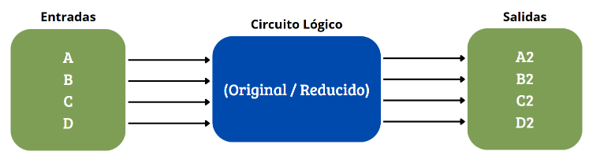
\includegraphics[width=0.5\textwidth]{Img/DiagramaDeBloques.png}
        \caption{Diagrama de bloques del funcionamiento del circuito.}
    \end{figure}

    A partir del análisis de las conexiones en el esquema del circuito original proporcionado por la guía de laboratorio, se determinaron las fórmulas matemáticas para cada una de las salidas:

    \begin{align*}
        A2 &= (AC) + (A + B) \\
        B2 &= (\boolnot{CD}) \cdot (B + D) \\
        C2 &= \boolnot{D} \\
        D2 &= (A + B) + C
    \end{align*}

    Donde las variables que componen el bloque combinacional corresponden a:

    \begin{itemize}
        \item \textbf{A: } Bits mas significativo de la entrada (MSB).
        \item \textbf{B y C: } Bits intermedios de la entrada.
        \item \textbf{D: } Bits menos significativo de la entrada (LSB).
        \item \textbf{A2: } Primera función de salida del convertidor de código.
        \item \textbf{B2: } Segunda función de salida del convertidor de código.    
        \item \textbf{C2: } Tercera función de salida del convertidor de código.
        \item \textbf{D2: } Cuarta función de salida del convertidor de código.
    \end{itemize}

    \subsection{Resultados esperados}

    Para demostrar el procedimiento matemático de evaluación de las expresiones y predecir los estados lógicos resultantes, se toma como caso de estudio el código de entrada binario ABCD = 0110.

    Donde:

    \begin{align*}
        A &= 0 \\
        B &= 1 \\
        C &= 1 \\
        D &= 0
    \end{align*}

    Evaluación de la ecuación (1):

    \begin{equation*}
        A2 = (0 \cdot 1) + (0 + 1) = 0 + 1 = 1 \longrightarrow \text{La luz se enciende}
    \end{equation*}

    Evaluación de la ecuación (2):

    \begin{equation*}
        B2 = (\boolnot{1 \cdot 0}) \cdot (1 + 0) = \boolnot{0} \cdot 1 = 1 \cdot 1 = 1 \longrightarrow \text{La luz se enciende}
    \end{equation*}

    Evaluación de la ecuación (3):

    \begin{equation*}
        C2 = \boolnot{0} = 1 \longrightarrow \text{La luz se enciende}
    \end{equation*}

    Evaluación de la ecuación (4):

    \begin{equation*}
        D2 = (0 + 1) + 1 = 1 + 1 = 1 \longrightarrow \text{La luz se enciende}
    \end{equation*}

    \subsection{Tabla de verdad del Circuito original}

    Repitiendo este mismo procedimiento de cálculo para las 16 combinaciones posibles de los interruptores de entrada, se construyó la Tabla 1, la cual detalla cuándo se enciende y se apaga cada luz en el primer circuito.

    \begin{table}[h]
    \centering
    \begin{tabular}{|c|c|c|c|c|c|c|c|}
    \hline
    A & B & C & D & A2 & B2 & C2 & D2 \\ \hline
    0 & 0 & 0 & 0 & 0 & 0 & 1 & 0 \\ \hline
    0 & 0 & 0 & 1 & 0 & 1 & 0 & 0 \\ \hline
    0 & 0 & 1 & 0 & 0 & 0 & 1 & 1 \\ \hline
    0 & 0 & 1 & 1 & 0 & 1 & 0 & 1 \\ \hline
    0 & 1 & 0 & 0 & 1 & 1 & 1 & 1 \\ \hline
    0 & 1 & 0 & 1 & 1 & 1 & 0 & 1 \\ \hline
    0 & 1 & 1 & 0 & 1 & 1 & 1 & 1 \\ \hline
    0 & 1 & 1 & 1 & 1 & 0 & 0 & 1 \\ \hline
    1 & 0 & 0 & 0 & 1 & 0 & 1 & 1 \\ \hline
    1 & 0 & 0 & 1 & 1 & 1 & 0 & 1 \\ \hline
    1 & 0 & 1 & 0 & 1 & 0 & 1 & 1 \\ \hline
    1 & 0 & 1 & 1 & 1 & 0 & 0 & 1 \\ \hline
    1 & 1 & 0 & 0 & 1 & 1 & 1 & 1 \\ \hline
    1 & 1 & 0 & 1 & 1 & 1 & 0 & 1 \\ \hline
    1 & 1 & 1 & 0 & 1 & 1 & 1 & 1 \\ \hline
    1 & 1 & 1 & 1 & 1 & 0 & 0 & 1 \\ \hline
    \end{tabular}
    \caption{Tabla de verdad del circuito original.}
    \label{tab:dVerdad}
    \end{table}

    \subsection{Simplificación de expresiones booleanas}

    El análisis del diseño consiste en la aplicación de los teoremas fundamentales del álgebra de Boole y las leyes de De Morgan sobre las ecuaciones obtenidas del circuito original. 

    Mediante este procedimiento matemático, se busca eliminar los términos redundantes para establecer las funciones mínimas que permitirán la construcción del Circuito Reducido

    \subsection{Simplificación y fórmulas para el Circuito Reducido}

    Con el fin de diseñar el circuito simplificado y optimizar el uso de componentes, se aplicaron los teoremas del álgebra de Boole de forma sucesiva en cada función original:

    \underline{Simplificación de la salida A2:}

    \begin{align*}
        A2 &= (AC) + (A + B) 
    \end{align*}

    Se eliminan los paréntesis de la suma mediante la propiedad asociativa:

    \begin{align*}
        A2 &= AC + A + B
    \end{align*}

    Se aplica la propiedad distributiva en el Álgebra de Boole $(A + AC = A)$ para eliminar el término $AC$: 

    \begin{align*}
        A2 &= A + B
    \end{align*}

    \underline{Simplificación de la salida B2:}

    \begin{align*}
        B2 &= (\boolnot{CD}) \cdot (B + D)
    \end{align*}

    Se transforma el primer término aplicando la primera Ley de De Morgan $(\boolnot{CD} = \boolnot{C} + \boolnot{D})$:

    \begin{align*}
        B2 &= (\boolnot{C} + \boolnot{D}) \cdot (B + D)
    \end{align*}

    Se realiza la multiplicación distributiva de los términos de ambos paréntesis:

    \begin{align*}
        B2 &= \boolnot{C}B + \boolnot{C}D + \boolnot{D}B + \boolnot{D}D
    \end{align*}

    Dado que una variable multiplicada por su inverso equivale a cero por ley de complementos $(\boolnot{D}D = 0)$, el termino se anula:

    \begin{align*}
        B2 &= \boolnot{C}B + \boolnot{C}D + \boolnot{D}B
    \end{align*}

    Ordenando los elementos, se establece la fórmula optimizada para el segundo circuito:

    \begin{align*}
        B2 &= B(\boolnot{C} + \boolnot{D}) + \boolnot{C}D
    \end{align*}

    \underline{Simplificación de la salida C2 y D2:}

    La función de la salida C2 ya se encuentra en su forma más simple, por lo que no requiere de ningún proceso de reducción:
    
    \begin{align*}
        C2 &= \boolnot{D}
    \end{align*}

    Por otro lado, la función de la salida D2 también se encuentra en su forma más simple, por lo que no requiere de ningún proceso de reducción:  

    \begin{align*}
        D2 &= (A + B) + C
    \end{align*}

    Al comparar las ecuaciones finales del Circuito Reducido ((5) y (6)) con las ecuaciones originales, se puede concluir que ambos sistemas realizarán exactamente la misma función lógica. Por este motivo, la tabla de verdad para ambos circuitos es la misma, de modo que los valores calculados previamente en la Tabla 1 sirven como los resultados esperados para validar tanto el circuito original como el simplificado en la etapa de simulación.

    %===========================================================================
    \newpage
    \section{Simulación del circuito}

    

    %===========================================================================
    \newpage
    \section{Conclusión}


\end{document}
